\documentclass[border=10pt]{standalone}

\usepackage{tikz}
\usetikzlibrary{arrows.meta,arrows,decorations.pathmorphing,backgrounds,positioning,fit,petri,calc,shapes.geometric,scopes,fit,spy}
\usepackage{pgfplots}
\pgfplotsset{,compat=1.11}
\tikzset{/pgf/number format/1000 sep={\,}}

\usepackage{fontawesome5}
\renewcommand{\familydefault}{\sfdefault}
\usepackage{helvet}

%%%%%%%%%%%%%%%%%%%%%%%%%%%%%%%%%%%%%%%%%%%%%%%%%%%%%%%%%%%%%%%%%%%%%%%%%%%%%%%%
% preamble
\providecommand{\hidText}[1]{$H_{#1}$}%
\makeatletter
\newcommand{\tikzANN@InputLayerTitle}{Input\\Layer}%
\newcommand{\tikzANN@HiddenLayerTitle}{Hidden\\Layer}%
\newcommand{\tikzANN@OutputLayerTitle}{Output\\Layer}%
\providecommand{\tikzANNInputLayerTitle} {\tikzANN@InputLayerTitle}%
\providecommand{\tikzANNHiddenLayerTitle}{\tikzANN@HiddenLayerTitle}%
\providecommand{\tikzANNOutputLayerTitle}{\tikzANN@OutputLayerTitle}%
\makeatother

\newcommand{\tikzANNResetTitleCommands}{%
\makeatletter
\renewcommand{\tikzANNInputLayerTitle} {\tikzANN@InputLayerTitle}%
\renewcommand{\tikzANNHiddenLayerTitle}{\tikzANN@HiddenLayerTitle}%
\renewcommand{\tikzANNOutputLayerTitle}{\tikzANN@OutputLayerTitle}%
\makeatother
}
\tikzset{synapseNode/.style={}}

%%%%%%%%%%%%%%%%%%%%%%%%%%%%%%%%%%%%%%%%%%%%%%%%%%%%%%%%%%%%%%%%%%%%%%%%%%%%%%%%
% varaibles
\renewcommand{\inText}[1]{
 $x_{#1}$
}
\renewcommand{\hidText}[1]{
 {$\sigma_{relu}(H_{#1})$}%
}
\renewcommand{\outText}[1]{
 $y_{#1}$%
}
\renewcommand{\synapseIHText}[2]{%
 {\ifthenelse{\equal{#1}{1}}{}{\small$W^{(I)}_{#1#2}$}}}
\renewcommand{\synapseHOText}[2]{\small$W^{(H)}_{#1#2}$}

%%%%%%%%%%%%%%%%%%%%%%%%%%%%%%%%%%%%%%%%%%%%%%%%%%%%%%%%%%%%%%%%%%%%%%%%%%%%%%%%
%main document
\begin{document}

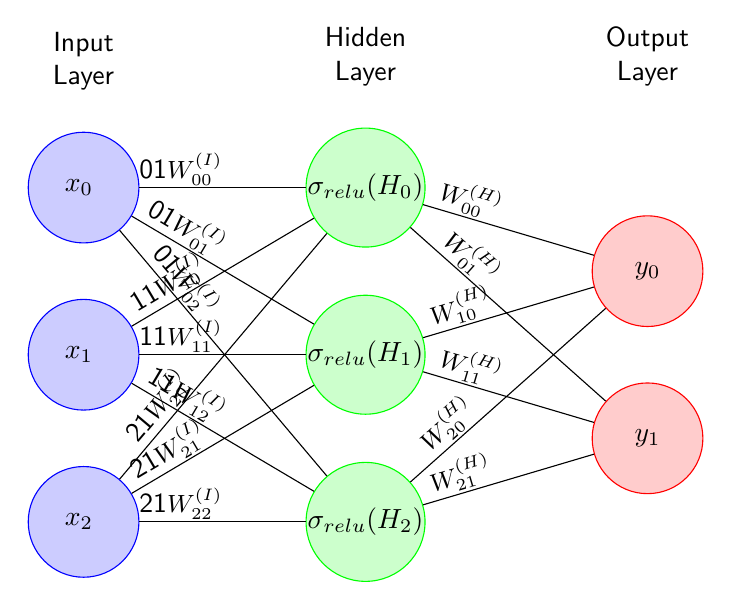
\begin{tikzpicture} [
  neuron/.style={circle,minimum size=4em,align=center},
  inNeuron/.style={neuron,draw=blue,fill=blue!20},
  hiddenNeuron/.style={neuron,draw=green,fill=green!20},
  outNeuron/.style={neuron,draw=red,fill=red!20},
  synapseNodeMy/.style={near start,sloped,above,
     outer sep=0ex,inner sep=.2ex, synapseNode},
  every node/.append style={node distance=2em,inner sep=0pt}
 ]
  \node[inNeuron] (in 0) {\inText{0}};
  \node[inNeuron, below=of in 0] (in 1) {\inText{1}};
  \node[inNeuron, below=of in 1] (in 2) {\inText{2}};

  \node[hiddenNeuron, right=6em of in 0] (hid 0) {\hidText{0}}; 
  \node[hiddenNeuron, right=6em of in 1] (hid 1) {\hidText{1}}; 
  \node[hiddenNeuron, right=6em of in 2] (hid 2) {\hidText{2}}; 

  \node[inner sep=0em,outer sep=0em, fit=(hid 0) (hid 1)] (hidG 01) {};
  \node[inner sep=0em,outer sep=0em, fit=(hid 2) (hid 1)] (hidG 12) {};

  \node[outNeuron, right=6em of hidG 01] (out 0) {\outText{0}}; 
  \node[outNeuron, right=6em of hidG 12] (out 1) {\outText{1}}; 

  \foreach \a in {0,...,2} {
   \foreach \s in {0,...,2} {
    \draw (in \a) -- (hid \s) node[synapseNodeMy] {\synapseIHText{\a}{\s}};
   }}

  \foreach \a in {0,...,2} {
   \foreach \s in {0,...,1} {
    \draw (hid \a) -- (out \s) node[synapseNodeMy] {\synapseHOText{\a}{\s}};
   }}

  \node[above=1.5em of in 0,align=center] {\tikzANNInputLayerTitle};
  \node[above=1.5em of hid 0,align=center] (hidTitle) {\tikzANNHiddenLayerTitle};
  \node[anchor=center,align=center] at (out 0 |- hidTitle) {\tikzANNOutputLayerTitle};


\end{tikzpicture}

\end{document}
